\documentclass[10pt]{article}
\usepackage{amsmath, amssymb, amsfonts}
\usepackage{amsthm}
\usepackage{graphicx}
\usepackage{hyperref}
\usepackage{geometry}
\geometry{margin=1in}
\usepackage{enumitem}
\usepackage{physics}
\usepackage{bm}
\usepackage{algorithm}
\usepackage{algpseudocode}
\usepackage{siunitx}
\usepackage{caption}
\usepackage{subcaption}

%  define custom commands
\newcommand{\R}{\mathbb{R}}
\newcommand{\N}{\mathbb{N}}
\newcommand{\Z}{\mathbb{Z}}
\newcommand{\E}{\mathbb{E}}
\newcommand{\Symmetric}{\mathbb{S}}
\newcommand{\diff}{\mathrm{d}}
\newcommand{\D}{\mathrm{d}}
\newcommand{\cov}[1]{\mathrm{Cov}[#1 ]}
\let\P\relax
\newcommand{\P}[1]{\mathbb{P}\left[#1\right]}
\let\E\relax
\newcommand{\E}[1]{\mathbb{E}\left[#1\right]}
\newcommand{\textr}{\textcolor{red}}
\newcommand{\textb}{\textcolor{blue}}
\newcommand{\suchthat}{\mathrm{s.t.}\quad}
\newcommand{\normal}{\mathcal{N}}
\newcommand{\indicator}{\mathds{1}}
\newcommand{\chol}[1]{(#1)^{\frac{1}{2}}}
\newcommand{\maxeig}[1]{\lambda_{\max} \left\{#1 \right\}}
\newcommand{\blkdiag}[1]{\mathrm{blkdiag}(#1)}
\newcommand{\diag}[1]{\mathrm{diag}(#1)}
\DeclareMathOperator*{\minimize}{minimize}


\newtheorem{theorem}{Theorem}
\newtheorem{assumption}{Assumption}
\newtheorem{problem}{Problem}
\newtheorem{remark}{Remark}

\usepackage{cleveref}
\crefname{align}{Eq.}{Eqs.}
\crefname{equation}{Eq.}{Eqs.}
\crefname{figure}{Fig.}{Figs.}
\crefname{table}{Table}{Tables}
\crefname{theorem}{Theorem}{Theorems}
\crefname{definition}{Definition}{Definitions}
\crefname{lemma}{Lemma}{Lemmas}
\crefname{remark}{Remark}{Remarks}
\crefname{assumption}{Assumption}{Assumptions}
\crefname{proof}{Proof}{Proofs}
\crefname{algorithm}{Algorithm}{Algorithms}
\crefname{problem}{Problem}{Problems}
\crefname{proposition}{Proposition}{Propositions}
\crefname{corollary}{Corollary}{Corollaries}
\crefname{section}{Section}{Sections}


\allowdisplaybreaks[1] %allows equations/align to span multiple pages

\newcommand\blfootnote[1]{%
  \begingroup
  \renewcommand\thefootnote{}\footnote{#1}%
  \addtocounter{footnote}{-1}%
  \endgroup
}

\def\showChanges{0} % Change this value to 1 (red) or 0 (black) to switch highlighting condition

% Define the highlighting command
\newcommand{\highlight}[1]{%
    \ifnum\showChanges=1
        \textcolor{red}{#1}%
    \else
        #1%
    \fi
}
% highlighting command for math mode, to preserve spacing
\newcommand{\mathhl}[1]{
    \ifnum\showChanges=1
        \mathcolor{red}{#1}
    \else
        #1
    \fi
}
\newcommand{\needsfix}[1]{%
    \textcolor{blue}{#1}%
}

\usepackage{marginnote}
\usepackage{tcolorbox}
\setlength{\marginparwidth}{0.8in}
\newcommand{\margincomment}[1]{%
    \ifnum\showChanges=1
    \textcolor{blue}{\setlength{\baselineskip}{10pt}\footnotesize\raggedright\marginnote{#1}}%
    \else
    \fi
}

% set path for figures
\graphicspath{{../figures/}}

\title{Square Root QR Covariance Steering}
\author{Naoya Kumagai}
\date{\today}

\begin{document}

\maketitle

\begin{abstract}
This document provides an overview and technical documentation for the Square Root QR Covariance Steering method, including problem formulation, algorithmic details, and implementation notes.
\end{abstract}

\section{Introduction}

Covariance steering is a control technique for steering the mean and covariance of a stochastic system to desired terminal values. The proposed square root QR approach improves numerical stability and efficiency, at the expense of an iterative algorithm.

\subsection{Notation and Preliminaries}
Let $\mathbb{L}_+^n$ denote the space of $n \times n$ lower triangular matrices with positive diagonal entries. 
The square root of a positive definite matrix \( P \in \mathbb{R}^{n \times n} \) is defined as the unique lower triangular matrix \( S \in \mathbb{L}_+^n \) such that \( P = S S^\top \). Its uniqueness is easily shown. $\mathrm{diag}(M)$ denotes the vector of diagonal elements of matrix \( M \). 


\begin{theorem}[Existence and Uniqueness of QR decomposition, Thm 3.3.3 in (cite)]
	Let \( M \in \mathbb{R}^{m \times n} \), \(m > n\). Then there exist \(Q \in \mathbb{R}^{m \times m}\) and \(\tilde{R} \in \mathbb{R}^{m \times n}\) such that \(Q\) is orthogonal, \( \tilde{R} = \begin{bmatrix}
	R \\ 0_{(m-n) \times n}
	\end{bmatrix}\), where \( R \in \mathbb{R}^{n \times n} \) is upper triangular, and
	\(M = QR\).
	Furthermore, if \(M\) has full rank, i.e. \(\mathrm{rank}(M) = n\), then the matrices \(Q\) and \(R\) are unique.
\end{theorem}
 If we require the diagonal entries of \( R \) to be positive, then $Q$ and $R$ are unique \cite{klosterHowUniqueQR}.

\subsection{Problem Formulation}
We address the finite-horizon discrete-time covariance steering problem for a linear time-varying system with additive Gaussian noise. The goal is to find a state feedback controller that steers the state covariance from an initial value to a desired terminal value while minimizing a cost function, and under chance constraints. Mathematically, the problem is formulated as follows.
\begin{subequations}
\label{eq:problem_statement}
\begin{align}
	\min_{\{K_k\}_{k=0}^{N-1}} \quad & J = \sum_{k=0}^{N-1} \mathbb{E} \left[ J_k (x_k, u_k)\right] \\
	\text{subject to} \quad & x_{k+1} = A_k x_k + B_k u_k + w_k, \quad k = 0, \ldots, N-1 \\
	& u_k = K_k x_k, \quad k = 0, \ldots, N-1 \\
	& x_0 \sim \mathcal{N}(\mu_0, P_{\mathrm{init}}) \\
	& P_N \leq P_f \\
	& \mathbb{P}(x_k \in \mathcal{X}_k) \geq 1 - \epsilon_k, \quad k = 0, \ldots, N \\ 
	& \mathbb{P}(u_k \in \mathcal{U}_k) \geq 1 - \delta_k, \quad k = 0, \ldots, N-1
\end{align}
\end{subequations}
where \( x_k \in \mathbb{R}^n \) is the state vector, \( u_k \in \mathbb{R}^m \) is the control input, \( w_k \in \mathbb{R}^n \) is zero-mean Gaussian process noise with covariance \( Q_k \), and \( K_k \in \mathbb{R}^{m \times n} \) is the state feedback gain to be designed. The matrices \( A_k \) and \( B_k \) define the system dynamics. We consider two types of cost functions:
\begin{equation}
	J_k (x_k, u_k) = \begin{cases}
		x_k^\top Q_k x_k + u_k^\top R_k u_k, \quad Q_k \geq 0, R_k > 0 & \text{(quadratic cost)} \\
		\norm{u_k}_2 & \text{(2-norm cost)}
	\end{cases}
\end{equation}

The sets \( \mathcal{X}_k \) and \( \mathcal{U}_k \) represent state and control constraints, respectively, with associated violation probabilities \( \epsilon_k \) and \( \delta_k \). We assume that the feasible region defined by the chance constraints is given in one of two forms: a linear constraint or a norm constraint. For the linear constraint form, the chance constraint can be expressed as:
\begin{equation} \label{eq:linear_chance_constraint}
	\mathbb{P}(\alpha_j ^\top x_k \leq \beta_j) \geq 1 - p_j
\end{equation}
for each linear constraint defined by \( \alpha_j \in \mathbb{R}^n \) and \( \beta_j \in \mathbb{R} \), with violation probability \( p_j \).
For the norm constraint form, the chance constraint can be expressed as:
\begin{equation} \label{eq:norm_chance_constraint}
	\mathbb{P}(\| x_k \|_2 \leq \gamma) \geq 1 - p_\gamma
\end{equation}
for some scalar \( \gamma > 0 \) and violation probability \( p_\gamma \). The same forms apply to the control input \( u_k \).

For convenience, we make the following assumption, which is reasonable in practical applications:
\begin{assumption} \label{assump:positive_definite_state}
	The state covariance remains strictly positive definite throughout the horizon.
\end{assumption}

\subsection{Relevant works}
The covariance steering problem has been well studied in the literature, and dates back to the early works by Hotz and Skelton \cite{hotzCovarianceControlTheory1987}. Recent works mainly focus on converting the problem into a
convex optimization problem. Skaf and Boyd \cite{skafDesignAffineControllers2010} considers a state-history feedback controller and formulates the problem as a semidefinite programming (SDP) problem. Okamoto et al. \cite{okamotoOptimalCovarianceControl2018} later adds chance constraints while maintaining convexity. However, these methods suffer from the poor computational complexity as the horizon length increases, due to the large linear matrix inequality (LMI) constraints involved \cite{rapakouliasDiscreteTimeOptimalCovariance2023a}. It is also important to note that the problem variables involve the ``square root'' of the covariance. 

A more recently proposed method by Liu et al. \cite{liuOptimalCovarianceSteering2024} uses the covariance directly as the optimization variable; in combination with an elegant proof of so-called ``lossless convexification'', it converts the seemingly nonconvex problem into an equivalent convex problem. Compared to the block approach, this method scales much better with the growth in problem size. At the same time, we have observed several drawbacks of this method: first, the numerical stability is not ideal as we are working with units that square the system units. Second, when dealing with objective functions or constraints that involve the covariance square root (e.g., the chance constraints), iterative algorithms are required. Third, due to the requirement of a proof of lossless convexification, whenever the problem formulation changes slightly, theoretical work is required to ensure the convexity of the new formulation.

\subsection{Contributions}



\section{Square root covariance propagation}

First, we provide a brief review of square root covariance propagation, mainly used for Kalman filtering \cite{tapleyStatisticalOrbitDetermination2004}. 
% In the 1960s, 
Let the system dynamics be given by:
\begin{equation}
	x_{k+1} = \Phi_k x_k + w_k
\end{equation}
with state \( x_k \in \mathbb{R}^n \), where \( w_k \in \mathbb{R}^m \) is zero-mean Gaussian noise with covariance \( Q_k \).
By defining $P_k := \E{(x_k - \E{x_k})(x_k - \E{x_k})^\top}$, the covariance propagation equation is given by:
\begin{equation}
	P_{k+1} = \Phi_k P_k \Phi_k^T + Q_k
\end{equation}
If we define \( S_k \in \mathbb{L}_+^n \) as \( S_k = P_k^{1/2} \) and \( V_k \in \mathbb{L}_+^m \) as \( V_k = Q_k^{1/2} \), the covariance propagation can be expressed as:
\begin{equation}
	S_{k+1} S_{k+1}^T = \Phi_k S_k S_k^T \Phi_k^T + V_k V_k^T = X_{k+1} X_{k+1}^T
\end{equation}
where we define
\begin{equation}
	X_{k+1} := \begin{bmatrix} \Phi_k S_k & V_k \end{bmatrix} \in \mathbb{R}^{n \times (n+m)}
\end{equation}
Note that the dimensions of $S_{k+1}$ and $X_{k+1}$ are different, so we cannot directly equate them.
To numerically obtain $S_{k+1}$ from $X_{k+1}$, we perform a QR decomposition
\textcolor{red}{Is this unique?}
:
\begin{equation}
	X_{k+1} Q_{k+1} = \begin{bmatrix} 0_{n \times m} & S_{k+1}^\top \end{bmatrix} 
\end{equation}
where \( Q_{k+1} \in \) is an orthogonal matrix.
In other words, the square root covariance propagation can be expressed as a nonlinear operation involving the QR decomposition:
\begin{equation}
	S_{k+1} = (\mathrm{qr}(X_{k+1}^\top))^\top = (\mathrm{qr}( \begin{bmatrix} \Phi_k S_k & V_k \end{bmatrix} ^\top))^\top
\end{equation}
where \( \mathrm{qr}(\cdot) \) denotes the operation of extracting the upper triangular factor \( R \) from the QR decomposition. 
In implementation, it is preferred to use the economy-size QR decomposition to avoid unnecessary computations. (This requires using $\mathrm{qr}(\cdot, \text{``econ"})$ in MATLAB.) In addition, to ensure uniqueness of the square root, if the function returns an \( R \) matrix with negative diagonal entries, we multiply the corresponding columns of \( Q \) and rows of \( R \) by -1 to ensure positive diagonals.

\subsection{QR decomposition derivative}
In order to use this square root covariance propagation in an optimization framework, we require the derivative of the QR decomposition operation; this is documented in the literature \cite{deleeuwDifferentiatingQRDecomposition2023}, but for completeness, we provide a brief overview here.
The derivative of the QR decomposition, i.e. the first-order perturbation analysis of the $R$ matrix with respect to perturbations in the $X$ matrix, is given by:
\begin{equation}
	A + (\dd R) R^{-1} = Q^\top (\dd X) R^{-1}
\end{equation}
where \( A \) is an antisymmetric (skew-symmetric) matrix such that 
\begin{equation}
	\mathrm{tril}(A) = \mathrm{tril}(Q^\top (\dd X) R^{-1}).
\end{equation}
\( \mathrm{tril}(A) \) replaces the upper triangular part of \( A \) with zeros.
Organizing the above, we have:
\begin{equation}
	\dd R = \dd R(\dd X, Q, R) := Q^\top (\dd X) - \mathrm{tril}(Q^\top (\dd X) R^{-1}) R.
\end{equation}
Thus, using the Taylor expansion, we can approximate the QR decomposition as a linear function of perturbations in \( X \), around some reference \( \bar{X} \):
\begin{equation}
	\mathrm{qr}(X) \approx \mathrm{qr}(\bar{X}) + \dd R(X - \bar{X}, Q(\bar{X}), R(\bar{X})).
\end{equation}
Note that \( \mathrm{qr}(X)\) and \(R(X)\) are synonymous.

\subsection{Application to Covariance Steering}
The application to covariance steering is straightforward.
Now, since the state is controlled by a feedback controller of the form
\begin{equation}
	u_k = K_k x_k,
\end{equation}
The closed-loop dynamics become
\begin{equation}
	x_{k+1} = (A_k + B_k K_k) x_k + w_k
\end{equation}
and the square root covariance propagation becomes
\begin{equation}
	S_{k+1} = (\mathrm{qr}(X_{k+1}^\top))^\top, \quad X_{k+1} = \begin{bmatrix} (A_k + B_k K_k) S_k & V_k \end{bmatrix}.
\end{equation}
Since both $P_k$ and $K_k$ are unknowns, there is a bilinear term \( K_k S_k \).
By defining $L_k = K_k S_k$, $K_k$ can be uniquely recovered as $K_k = L_k S_k^{-1}$. The inverse exists when the diagonals of $S_k$ are non-zero, which is by definition
guaranteed since $S_k$ is the square root of a positive definite covariance matrix (\(\because\) \cref{assump:positive_definite_state}).
So we get
\begin{equation} \label{eq:square_root_covariance_propagation}
	S_{k+1} = (\mathrm{qr}(X_{k+1}^\top))^\top, \quad X_{k+1} = \begin{bmatrix} (A_k S_k + B_k L_k) & V_k \end{bmatrix}.
\end{equation}
with its first-order approximation given by:
\begin{equation} \label{eq:square_root_covariance_propagation_linearized}
	S_{k+1} \approx (\mathrm{qr}(\bar{X}_{k+1}^\top))^\top + \left( \dd R(X_{k+1} - \bar{X}_{k+1}, Q(\bar{X}_{k+1}), R(\bar{X}_{k+1})) \right)^\top
\end{equation}
where \( \bar{X}_{k+1} = \begin{bmatrix} A_k \bar{S}_k + B_k \bar{L}_k & V_k \end{bmatrix} \), \(\bar{S}_k\) and \(\bar{L}_k\) being the reference variables.

\subsection{Objective function}
After substituting \( u_k = K_k x_k = L_k S_k^{-1} x_k \), and some standard manipulations, the objective function can be expressed as deterministic convex functions of \( L_k \) and \( S_k \):
\begin{equation} \label{eq:objective_deterministic}
	J = \begin{cases}
	\sum_{k=0}^{N-1} \mathrm{trace} (Q_k S_k S_k^\top + R_k L_k L_k^\top) & \text{(quadratic cost)} \\
	\sum_{k=0}^{N-1} \norm{L_k}_2 & \text{(2-norm cost)}.
	\end{cases}
\end{equation}

\subsection{Constraints}
The initial covariance constraint $P_0 = P_{\mathrm{init}}$ is imposed by:
\begin{equation} \label{eq:initial_covariance_deterministic}
	S_0 = P_{\mathrm{init}}^{1/2}
\end{equation}
The terminal covariance constraint $P_N \leq P_f$ is imposed by:
\begin{equation} \label{eq:terminal_covariance_deterministic}
	\norm{P_f^{-1/2} S_N}_2 - 1 \leq 0
\end{equation}
where \( \norm{\cdot}_2 \) denotes the spectral norm.
To ensure uniqueness of the square root, we impose:
\begin{equation} \label{eq:S_diagonals_positive}
	\mathrm{diag}(S_k) \geq 0, \quad \text{k = 0, \ldots, N}
\end{equation}

Since we are working with the square root form, chance constraints can also be imposed in a convex manner.
For the linear constraint form \eqref{eq:linear_chance_constraint}, the chance constraint can be exactly expressed as:
\begin{equation} \label{eq:linear_chance_constraint_deterministic}
	\alpha_j^\top \mu_k + \Phi^{-1}(1 - p_j) \norm{S_k^\top \alpha_j}_2 - \beta_j \leq 0
\end{equation}
where \( \Phi^{-1}(\cdot) \) is the inverse of the standard normal cumulative distribution function.
For the norm constraint form \eqref{eq:norm_chance_constraint}, the chance constraint can be conservatively approximated as:
\begin{equation} \label{eq:norm_chance_constraint_deterministic}
	\norm{\mu_k}_2 + \sqrt{Q_{\chi^2_n}(1 - p_\gamma)} \norm{S_k}_2 - \gamma \leq 0
\end{equation}
where \( Q_{\chi^2_n}(\cdot) \) is the inverse of the chi-squared cumulative distribution function with \( n \) degrees of freedom.
The control chance constraints can be imposed by replacing \( \mu_k \) with \( v_k \) and \( S_k \) with \( L_k \).

To summarize, \eqref{eq:problem_statement} is converted into a nonconvex optimization problem as follows:
\begin{equation}
	\min_{L_{0:N-1}, S_{0:N}} \eqref{eq:objective_deterministic} \quad \text{subject to} \quad \eqref{eq:square_root_covariance_propagation}, \eqref{eq:initial_covariance_deterministic}, \eqref{eq:terminal_covariance_deterministic}, \eqref{eq:S_diagonals_positive}, \eqref{eq:linear_chance_constraint_deterministic}, \eqref{eq:norm_chance_constraint_deterministic}
\end{equation}

\section{Algorithm Overview}
In order to take advantage of the convex representation of the objective and constraints, we use sequential convex programming (SCP). In the implementation, the first order approximation of the covariance propagation \eqref{eq:square_root_covariance_propagation_linearized} is imposed in a vectorized form with penalization of violations:
\begin{equation}
	\mathrm{vectril} \left\{ S_{k+1} - (\mathrm{qr}(\bar{X}_{k+1}^\top))^\top - \left( \dd R(X_{k+1} - \bar{X}_{k+1}, Q(\bar{X}_{k+1}), R(\bar{X}_{k+1})) \right)^\top \right\} = \chi_k
\end{equation}
where $\mathrm{vectril}(\cdot)$ vectorizes the lower triangular part of a matrix, and \( \chi_k \in \mathbb{R}^{\frac{n(n-1)}{2}}\) is a slack variable, penalized in the objective function via an Augmented Lagrangian method \cite{oguriSuccessiveConvexificationFeasibility2023a}. By using the specific SCP algorithm $\texttt{SCvx*}$, we can ensure that 1. the nonlinear dynamics are obeyed at convergence, and 2. the converged solution is locally optimal. As seen in our numerical experiments, the convergence is well-behaved, and compared to the globally optimal solution obtained from the full covariance steering method, the cost function values match to high precision.

\section{Numerical Examples}
Use the same problem parameters as in Liu's paper. The convex optimization problems are solved in MATLAB using YALMIP \cite{lofbergYALMIPToolboxModeling2004} and MOSEK \cite{mosekapsMOSEKOptimizationToolbox2025}. We use the same SCP parameters as in \cite{oguriSuccessiveConvexificationFeasibility2023a}.

Some practical implementation tips:
\begin{itemize}
	\item Since the algorithm requires iteratively linearizing the problem, an initial guess is required for each of the variables. The initial guess for \( S_k \) can be obtained by linearly interpolating between the Cholesky factors of the initial and terminal covariances. The initial guess for \( L_k \) can be set to zero.
	\item The SCP algorithm allows the user to choose whether to impose a trust region on the variables, to ensure that the solution remains in a region where the linear approximation is accurate. We observed that a trust region on \( L_k\) is not necessary, and causes chattering close to the solution.
\end{itemize}

\subsection{Comparison with Full Covariance Approach}
The cost function value match to 7 digits between the full covariance steering and the square root QR covariance steering methods.

%  plot the two results side by side
\begin{figure}[h]
	\centering
	\begin{subfigure}[b]{0.45\textwidth}
		\centering
		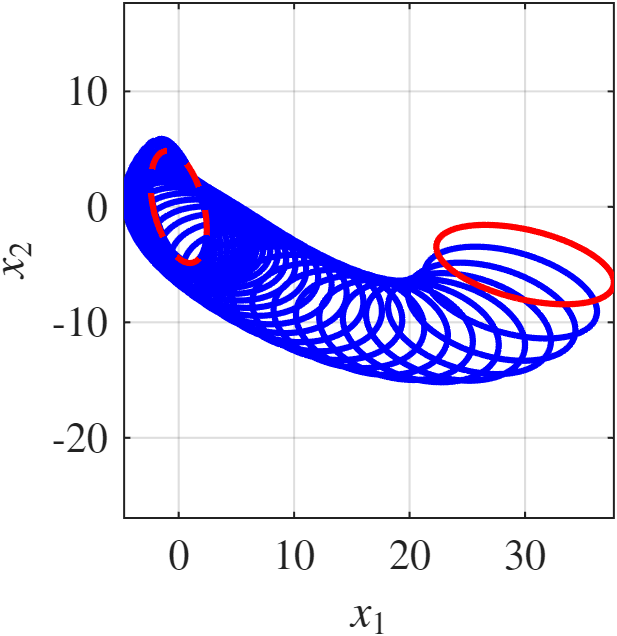
\includegraphics[width=\textwidth]{full_covariance_steering_result.png}
		\caption{Full covariance steering result}
		\label{fig:full_cov_result}
	\end{subfigure}
	\hfill
	\begin{subfigure}[b]{0.45\textwidth}
		\centering
		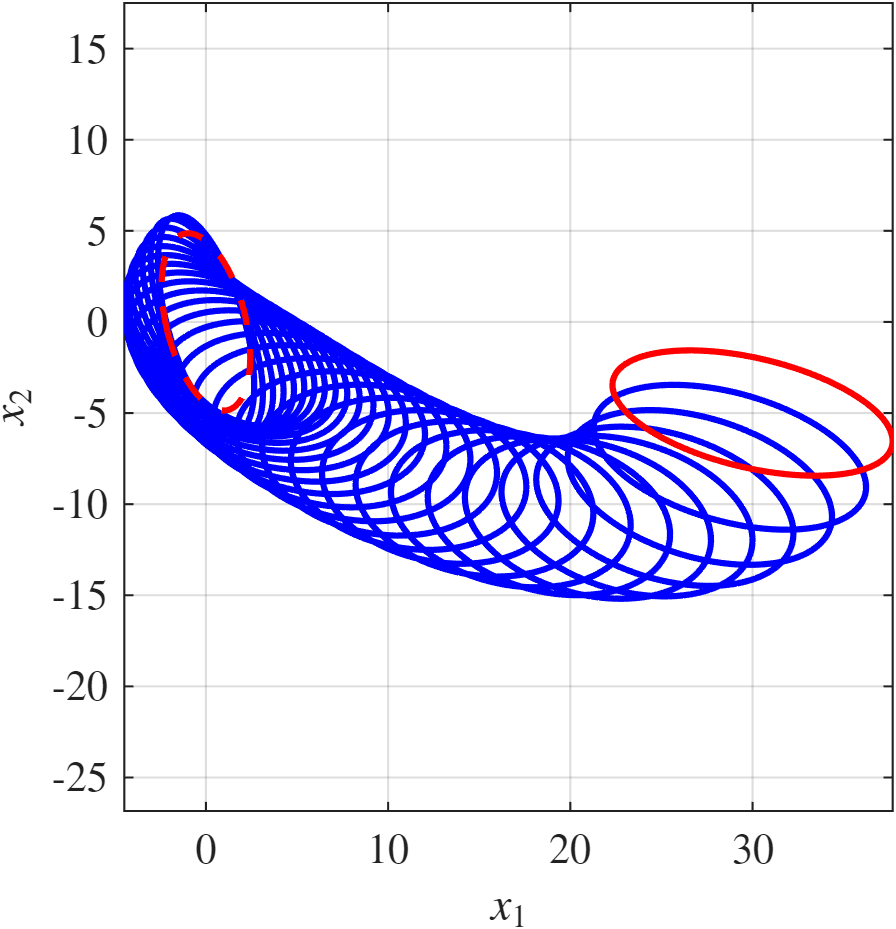
\includegraphics[width=\textwidth]{sqrt_covariance_steering_result.png}
		\caption{Square root QR covariance steering result}
		\label{fig:sqrt_qr_cov_result}
	\end{subfigure}
	\caption{Comparison of covariance steering results}
	\label{fig:cov_steering_comparison}
\end{figure}

\begin{figure}[h]
	\centering
	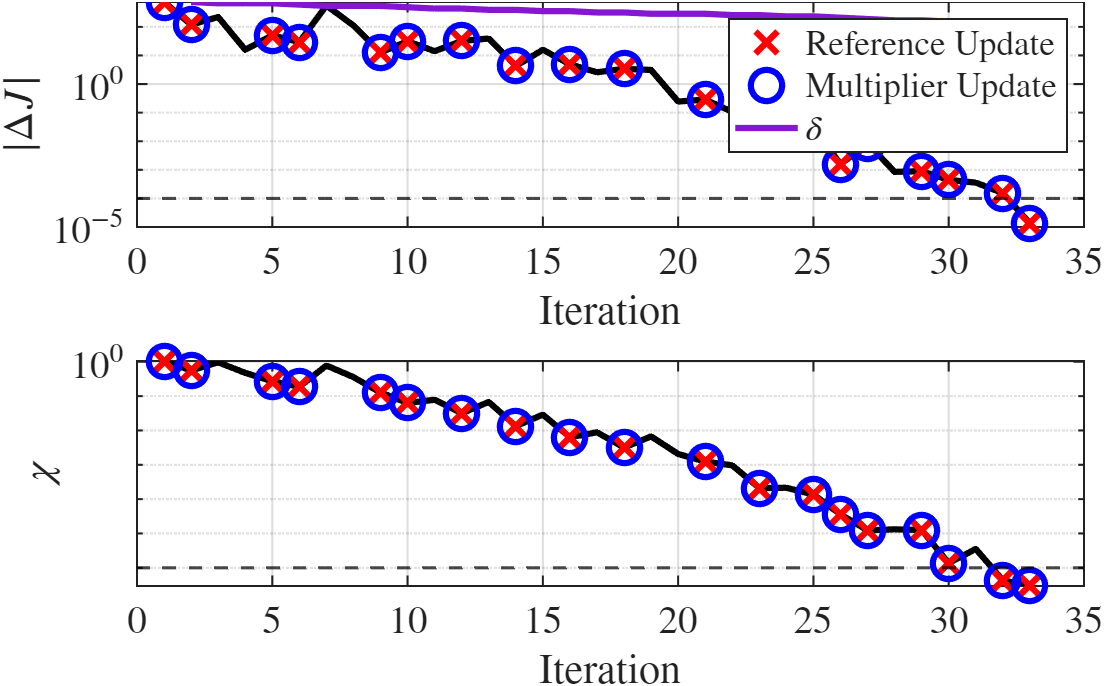
\includegraphics[width=0.6\textwidth]{sqrt_covariance_steering_convergence.png}
	\caption{Convergence history of the \textit{SCvx*} algorithm for the proposed method}
	\label{fig:sqrt_qr_cov_convergence}
\end{figure}


\subsection{Chance constraints}
Showcase the chance constraints handling capability and compare solution times with full covariance and block approaches.

\section{Conclusions}


% \section{Acknowledgements}
% This material is based upon work supported by the Air Force Office of Scientific Research under award number FA9550-23-10512. N. Kumagai acknowledges support for his graduate studies from the Shigeta Education Fund.

\clearpage
\bibliographystyle{plain}
\bibliography{references}


\end{document}
